
\section{Neural Networks}

\subsection{Architectures}

We compare five different network architectures,
which are all inspired by \cite{lecun98}.

\subsubsection{Layer types}

First note that a 32x32-pixel image with 3 colour-channels from the CIFAR-10 dataset is represented
by a matrix with dimensions (3, 32, 32).
We call the first dimension ``depth'' (i.e. the number of channels) and the other two dimensions ``height'' and ``width''.\\
Analogue, grayscaled images of the ZIP dataset have shape (1, 16, 16)
and images of the MNIST dataset have shape (1, 28, 28).\\

Each layer of a neural network takes an image representation matrix as input and transforms it to
another representation with a potentially different dimensions.
In the following we explain how that works for the three layer types that we use,
namely dense layers, convolution layers and subsampling layers.\\

\textbf{Dense layer}\\

Each neuron of a dense layer is connected to all the values of the layer's input.
A dense layer with $k$ neurons produces an output of dimensions ($k$, 1, 1), independent from the input shape.\\
In this work we always use the RelU activation function for dense layers.\\
Each of our networks has a dense layer with 10 neurons as last layer,
where the activation of a neuron stands for the score for one of the
10 classes.\\

\textbf{Convolution layer}\\

A convolution layer has $f$ filters with filter shape ($s$, $s$).
Each neuron is connected fully in depth to the input, but is only connected to a field of size ($s$, $s$)
in width and height of the input.\\
A convolution layer with input shape ($d$, $h$, $w$) produces an output with shape ($f$, $h-s+1$, $w-s+1$).\\

\textbf{Subsampling layer}\\

A subsampling layer reduces the width and height of the image representation,
but conserves its depth.
We use maximum subsampling with a stride of size (2, 2), which means each neuron of the subsampling layer
creates the maximum value of 4 input values as output.
By doing so, a subsampling layer with input shape ($d$, $h$, $w$) produces an output with shape ($d$, $h/2$, $w/2$).

\subsubsection{Dense networks}

We compare three networks which only have dense layers.\\

\textbf{Dense300}\\

The first of these networks has only one single dense layer with 300 neurons.
It is meant to be a rather simple baseline, that should be beaten by the other networks.\\

\textbf{Dense1000}\\

This network has one dense layer with 1000 neurons.
By comparing its performance with the Dense300-network, we can see whether an increase of the number of neurons
leads to better results.\\

\textbf{Dense300-100}\\

This network has two sequential dense layers with 300 and 100 neurons.
By comparing its performance with the Dense300-network, we can see whether an increase of the
depth\footnote{Note that when talking about networks the term ``depth'' refers to the number of layers,
but when talking about convolution layers it means the number of filters.}
of the network
leads to better results.

\subsubsection{Lenet1}

This network architecture is similar to the one named ``lenet1''
in \cite{lenet1}.\\

It has the following layers:\\

\begin{tabular}{|l|c|}
 \hline
 layer & output shape\\ \hline
 input image shape & (3, 32, 32)\\
 convolution layer with 4 filters of size (5, 5) & (4, 28, 28)\\
 subsampling layer & (4, 14, 14)\\
 convolution layer with 12 filters of size (5, 5) & (12, 10, 10)\\
 subsampling layer & (12, 5, 5)\\
 convolution layer with 10 filters of size (5, 5) & (10, 1, 1)\\
 output layer (dense) & (10, 1, 1)\\ \hline
\end{tabular}\\

When using this network on the ZIP data, we had to remove the
two subsampling layers, in order to match the smaller width
and height of the input images.\\
For the same reason, the second subsampling layer was removed when
dealing with the MNIST dataset.

\subsubsection{Lenet5}

This network is similar to the one named ``lenet5'' from \cite{lecun98},
which was especially designed for the MNIST dataset.\\

The structure is the following:\\

\begin{tabular}{|l|c|}
 \hline
 layer & output shape\\ \hline
 input image shape & (3, 32, 32)\\
 convolution layer with 6 filters of size (5, 5) & (6, 28, 28)\\
 subsampling layer & (6, 14, 14)\\
 convolution layer with 16 filters of size (5, 5) & (16, 10, 10)\\
 subsampling layer & (16, 5, 5)\\
 convolution layer with 120 filters of size (5, 5) & (120, 1, 1)\\
 dense layer with 84 neurons & (84, 1, 1)\\
 output layer (dense) & (10, 1, 1)\\ \hline
\end{tabular}\\

Lenet5 is similar to lenet1, but has convolution layers with more filters
and an additional dense layer in the end.\\

For the CIFAR-10 dataset we used the architecture as described above.\\
We had to adapt the structure for the MNIST dataset,
because \cite{lecun98} had 32x32-pixel versions of images
whereas our images are of size 28x28.
It was enough to reduce the filter size
of the last convolutional layer from (5, 5) to (4, 4) in order
to make the network applicable to the smaller input images.\\
When using it for the ZIP dataset, the filters stayed unchanged
but we again had to remove the subsampling layers.\\


\subsection{Results}

We kept $1/3$ of the training set of each dataset as a validation set and trained the networks
on a smaller training set of only $2/3$ of its size.
We then evaluated the performance of the networks on the validation sets in order to decide
which network architecture is the best one for each of the datasets.
Only in the end the chosen network was trained on the full training set and evaluated on the test set.\\

For the first training phase with the smaller training set we provide a plot
that shows how the accuracy on the training set and the accuracy on the validation set evolve over
100 training iterations (i.e. the network sees each training image 100 times).\\
The plot shows the training accuracies as dots and the validation accuracies as lines.\\
This evaluation shows us which network performs best and until which iteration the training and validation accuracies
increase.\\

We provide another plot that shows the validation accuracy over the training accuracy for each iteration.\\
When the points in this plot are close to the diagonal from (0,0) to (1,1), we consider this as a good learning process,
because the training accuracy and the validation accuracy increase with the same pace.\\
When the points range from left to right, the training accuracy increases but the network does not generalize to new data
and therefore the validation accuracy stays the same.\\
When the points move to the right and downwards, this is a sign that overfitting happens,
i.e. the training accuracy increases but the validation accuracy becomes worse.


\subsubsection{ZIP dataset}

See the plots of the training process in Figure \ref{zip_plots}.\\
All the five networks perform nearly equally well, only lenet5 is better than the others by a small margin.

\begin{tabular}{|l|c|c|}
 \hline
 network & best valid. acc. & at iteration\\ \hline
 dense300 & 96.95 \% & 83\\
 dense1000 & 96.87 \% & 94\\
 dense300-100 & 97.28 \% & 95\\
 lenet1 & 97.28 \% & 76\\
 lenet5 & \textbf{98.39} \% & 84\\
 \hline
\end{tabular}

\begin{figure}
 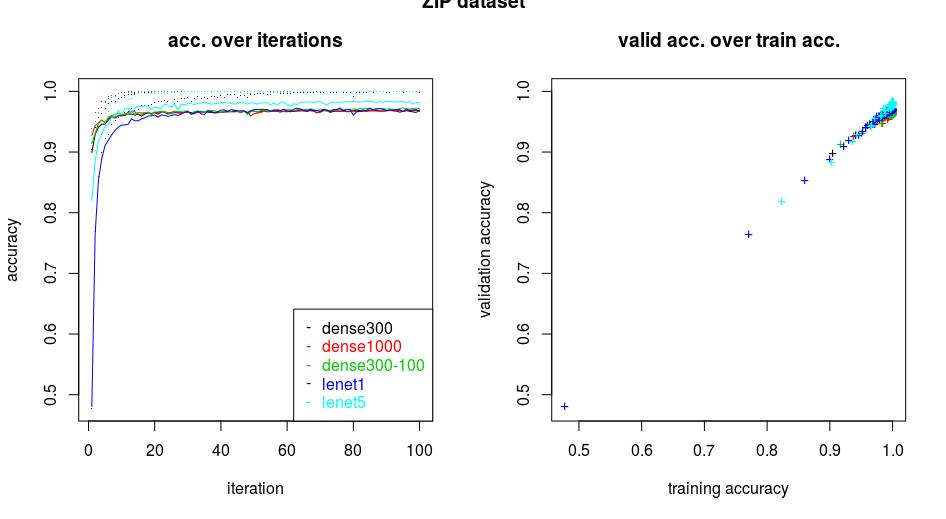
\includegraphics[width=\textwidth]{../plots/nn_zip}
 \caption{Evaluation of the neural networks on the ZIP dataset.}
 \label{zip_plots}
\end{figure}


\subsubsection{MNIST dataset}

See the plots of the training process in Figure \ref{mnist_plots}.\\
We observe that lenet5 behaves best on the MNIST dataset,
followed by lenet1.\\
The dense networks are a little bit worse.
The best dense network is dense1000, whereas the others perform nearly equally well.\\

\begin{tabular}{|l|c|c|}
 \hline
 network & best valid. acc. & at iteration\\ \hline
 dense300 & 98.04 \% & 35\\
 dense1000 & 98.23 \% & 96\\
 dense300-100 & 98.06 \% & 45\\
 lenet1 & 98.65 \% & 88\\
 lenet5 & \textbf{99.12} \% & 87\\
 \hline
\end{tabular}

\begin{figure}
 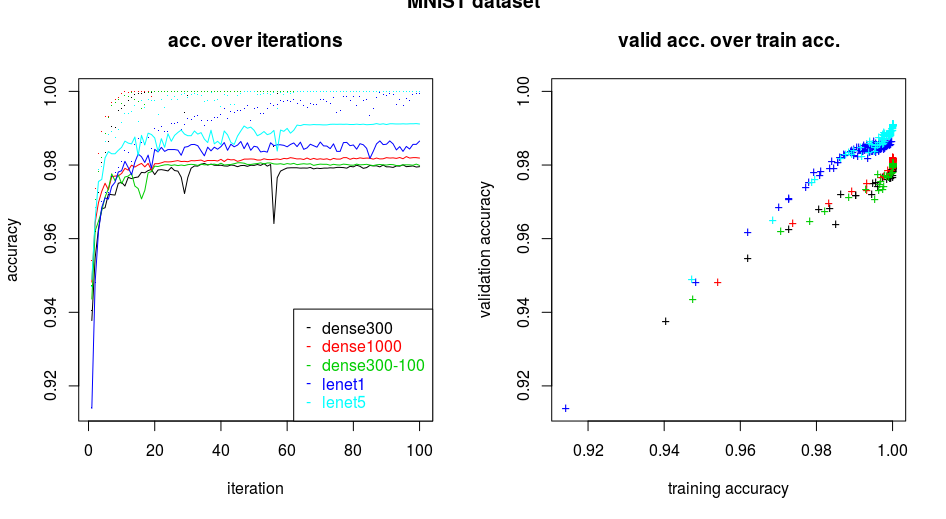
\includegraphics[width=\textwidth]{../plots/nn_mnist}
 \caption{Evaluation of the neural networks on the MNIST dataset.}
 \label{mnist_plots}
\end{figure}


\subsubsection{CIFAR-10 dataset}

See the plots of the training process in Figure \ref{cifar10_plots}.\\
We observe that lenet5 beats the other networks by a huge margin,
but starts to overfit after 30 iterations.\\
Lenet1 has a constant learning curve, whereas the dense networks
get stuck and do no longer improve after several iterations.\\

\begin{tabular}{|l|c|c|}
 \hline
 network & best valid. acc. & at iteration\\ \hline
 dense300 & 50.46 \% & 61\\
 dense1000 & 51.16 \% & 28\\
 dense300-100 & 50.08 \% & 46\\
 lenet1 & 56.15 \% & 99\\
 lenet5 & \textbf{61.15} \% & 37\\
 \hline
\end{tabular}\\

\begin{figure}
 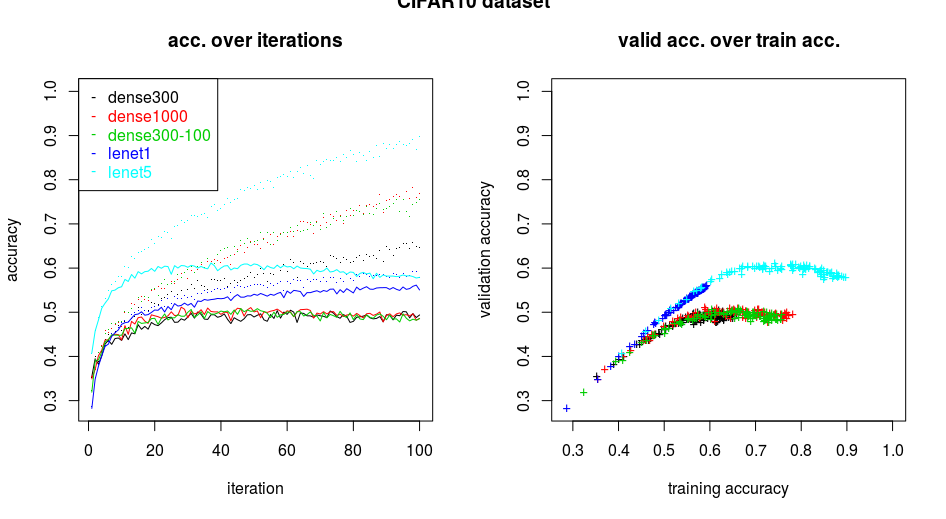
\includegraphics[width=\textwidth]{../plots/nn_cifar10}
 \caption{Evaluation of the neural networks on the CIFAR-10 dataset.}
 \label{cifar10_plots}
\end{figure}

\textbf{More filters}\\

Since the validation accuracies on the CIFAR-10 dataset are not very good, we try to improve the lenet5
network by adding more filters to each convolution layer.\\

After 30 iterations we get the following results:\\

\begin{tabular}{|c|c|c|}
 \hline
 network(filters) & training accuracy & validation accuracy\\ \hline
 lenet5(6,16,120) & 71.02 \% & 60.29 \% \\
 lenet5(16,32,120) & 84.31 \% & 65.85 \% \\
 lenet5(32,64,256) & 97.42 \% & \textbf{67.15} \% \\
 \hline
\end{tabular}\\

We observe that adding more filters increases the validation accuracy
by some points, but has a higher effect on the training accuracy.


\subsection{Final results and state of the art}

Finally, we trained the models selected above on the whole training
set of each dataset and compare the test accuracy with
the state of the art results listed on \cite{state-of-art}.\\

\begin{tabular}{|c|c|c|}
 \hline
 network(filters):iterations @ dataset & test accuracy & state of the art\\ \hline
 lenet5(6,16,120):40 @ ZIP & 94.71 \% & - \\
 lenet5(6,16,120):70 @ MNIST & ?? \% & 99.79 \% \\
 lenet5(32,64,256):30 @ CIFAR-10 & ?? \% & 96.53 \% \\
 \hline
\end{tabular}
